\documentclass{article}
\usepackage[catalan]{babel}
\usepackage[latin1]{inputenc}   % Permet usar tots els accents i car�ters llatins de forma directa.
\usepackage{enumerate}
\usepackage{amsfonts, amscd, amsmath, amssymb}
\usepackage[pdftex]{graphicx}

\setlength{\textwidth}{16cm}
\setlength{\textheight}{24.5cm}
\setlength{\oddsidemargin}{-0.3cm}
\setlength{\evensidemargin}{0.25cm} \addtolength{\headheight}{\baselineskip}
\addtolength{\topmargin}{-3cm}

\newcommand\Z{\mathbb{Z}}
\newcommand\R{\mathbb{R}}
\newcommand\N{\mathbb{N}}
\newcommand\Q{\mathbb{Q}}
\newcommand\K{\Bbbk}
\newcommand\C{\mathbb{C}}

\newcounter{exctr}
\newenvironment{exemple}
{ \stepcounter{exctr} 
\hspace{0.2cm} 
\textit{Exemple  \arabic{exctr}: }
\it
\begin{quotation}
}{\end{quotation}}


\begin{document}

\noindent
\textbf{Sistemes Invariants en el Temps}

\vskip 0.3 cm
\noindent
Un sistema es diu \textbf{invariant en el temps} (IT) si
a una entrada retardada en el temps li correspon una
sortida amb el mateix retard temporal. \'Es a dir:
\[
\text{si } y[n]={\cal T}(x[n]) \qquad \text{llavors} \qquad
y[n-k]={\cal T}(x[n-k])
\]

\noindent
Si un sistema ${\cal T}$  \'es invariant en el temps llavors els seg\"uents diagrames de blocs 
s\'on equivalents:

\vskip 0.3 cm
\begin{center}
\begin{tabular}{ccc}
\begin{minipage}{6cm}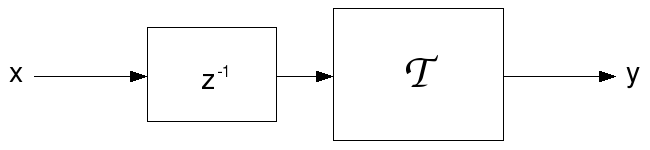
\includegraphics[width=6cm]{tinvariant1.png}\end{minipage}
 & $\qquad$ &
\begin{minipage}{6cm}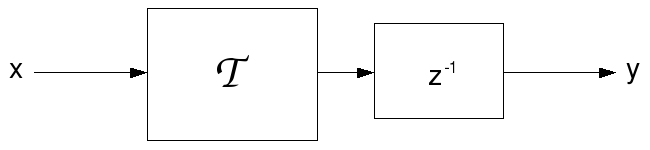
\includegraphics[width=6cm]{tinvariant2.png}\end{minipage}
\end{tabular}
\end{center}

\vskip 0.3 cm
\noindent
Exemple: 

�s el sistema $y[n]={\cal T}(x[n])=x[-n]$ invariant en el temps?

\vskip 0.3 cm
\noindent
Entrada: $x[n-k]$

\vskip 0.3 cm
\noindent
Sortida: si anomenam $z[n]=x[n-k]$, llavors ${\cal T}(x[n-k])={\cal T}(z[n])=z[-n]=x[-n-k]$

\vskip 0.3 cm
\noindent
Sortida si el sistema �s IT: $y[n-k]=x[-(n-k)]=x[-n+k]$

\vskip 0.3 cm
\noindent
Com que $y[n-k] \neq {\cal T}(x[n-k])$ llavors \textbf{el sistema no �s TI}.


\vskip 0.5 cm
\noindent
Si per exemple $x=\{-2, \underline{0}, 1 \}$ i $k=1$:

\begin{figure}[htbp]

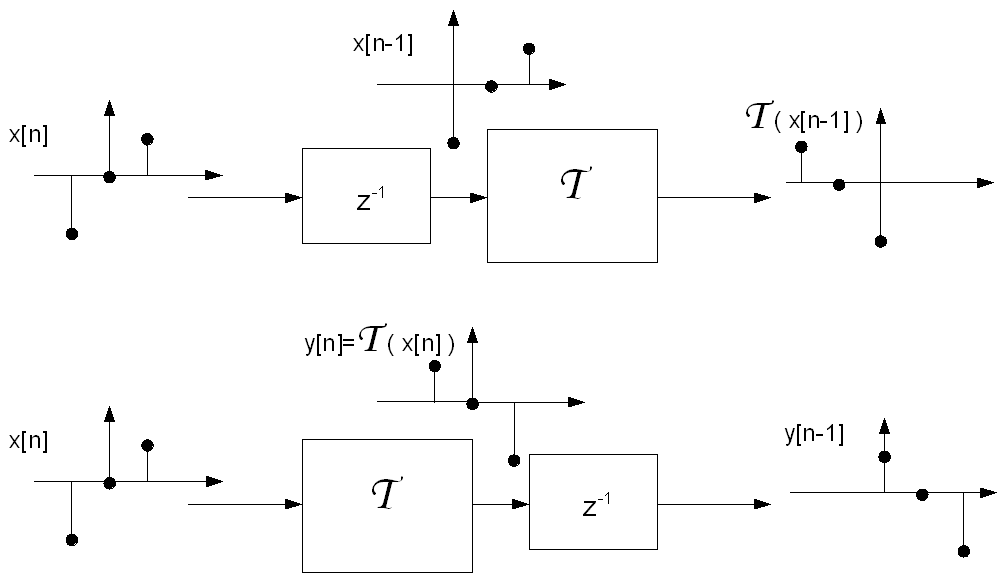
\includegraphics[width=16cm]{exIT.png} 

\end{figure}








\end{document}

